%\documentclass[twoside,twocolumn,9pt]{article}
\documentclass[journal=jcisd8,manuscript=article,layout=twocolumn]{achemso}

%\usepackage[super,sort&compress,comma]{natbib}
\usepackage{natbib}
%\usepackage[left=1.5cm, right=1.5cm, top=1.785cm,bottom=2.0cm]{geometry}
\usepackage[english]{babel}
\usepackage[T1]{fontenc}
\usepackage{hyperref}
\usepackage{graphicx}
\graphicspath{{./figures}{../figures}}
\usepackage{xcolor}

\usepackage{booktabs}
\usepackage{multirow}
\usepackage{amsmath}

\usepackage{epstopdf}


%% color
\usepackage{ulem}


\SectionNumbersOn

\title{Size Matters: free-energy calculations of amino acid adsorption over pristine graphene}


%%%%%%%%%%%%%%%%%%%%%%%%%%%%%%%%%%%%%%%%%%%%%%%%%%%%%%%%%%%%%%%%%%%%%
%% Meta-data block
%% ---------------
%% Each author should be given as a separate \author command.
%%
%% Corresponding authors should have an e-mail given after the author
%% name as an \email command. Phone and fax numbers can be given
%% using \phone and \fax, respectively; this information is optional.
%%
%% The affiliation of authors is given after the authors; each
%% \affiliation command applies to all preceding authors not already
%% assigned an affiliation.
%%
%% The affiliation takes an option argument for the short name.  This
%% will typically be something like "University of Somewhere".
%%
%% The \altaffiliation macro should be used for new address, etc.
%% On the other hand, \alsoaffiliation is used on a per author basis
%% when authors are associated with multiple institutions.
%%%%%%%%%%%%%%%%%%%%%%%%%%%%%%%%%%%%%%%%%%%%%%%%%%%%%%%%%%%%%%%%%%%%%
\author{Mateo Barria-Urenda}
\affiliation{Centro Interdisciplinario de Neurociencia de Valparaíso.}
\alsoaffiliation{Doctorado en Ciencias, Mención Biofísica y Biología Computacional, Facultad de Ciencias, Universidad de Valparaíso}
\alsoaffiliation{Millennium Nucleus in NanoBioPhysics (NNBP)}
\author {Alvaro Ruiz-Fernandez}
\affiliation{Centro Científico y Tecnológico de Excelencia Ciencia \& Vida.}
\author{Carlos Gonzalez}
\affiliation{Millennium Nucleus in NanoBioPhysics (NNBP)}
\alsoaffiliation{}
\author{Chris Oostenbrink}
\affiliation{Institute for Molecular Modeling and Simulation, University of Natural Resources and
Life Sciences, 1190 Vienna, Austria.}

\author{Jose Antonio Garate}
\affiliation{Facultad de Ingeniería, Arquitectura y Diseño, Universidad San Sebastián, Bellavista , Santiago, Chile.}
\alsoaffiliation{Millennium Nucleus in NanoBioPhysics (NNBP)}
\alsoaffiliation{Centro Científico y Tecnológico de Excelencia Ciencia \& Vida.}
\alsoaffiliation{Centro Interdisciplinario de Neurociencia de Valparaíso.}


\email{jose.garate@uss.cl}


\begin{document}

\maketitle

\abstract{
There is a still growing interest in graphene interactions with proteins; both for its possible biological applications and due to concerns over detrimental effects at the cellular level.
As with any process involving proteins, an understanding from amino acid composition is desirable.
In this work we systematically studied the adsorption process of amino acids onto pristine graphene via rigurous free-energy calculations.
We characterized the free energy, potential energy, and entropy of adsorption of all proteinogenic amino acids.
The energetic components were further separated into pair interaction contributions.
A linear correlation was found between the free-energy and the Solvent Accessible Surface Area  change  during adsorption($\Delta$SASA$^{ads}$).
Free energies over pristine graphene were compared with adsorption onto graphene oxide (GO), finding an almost complete loss of the favorability of amino acid adsorption onto graphene.
Finally, the correlation with the $\Delta$SASA$^{ads}$ was used to successfully predict the free-energy of adsorption of penta-L-alanine in two different structural states.
Due to the relative ease of calculating the ($\Delta$SASA$^{ads}$ compared to free-energy calculations, it could prove a cost-effective predictor of the free-energy of adsorption for proteins onto non-polar surfaces.
}

\section{Introduction}

% Context
%https://www.hindawi.com/journals/bmri/2021/5518999/
% http://graphenetimes.com/2009/12/boehms-1961-isolation-of-graphene/

Pristine graphene is a mono-layer molecule formed by a honeycomb lattice of aromatic carbons. First observed by Boehm in 1964\cite{Boehm_1962} and synthesized in 2004, \cite{Novoselov_2004} graphene has since experienced an explosive growth in interest. \cite{Randviir_2014}
In particular for graphene and its derivatives, many biological applications have been proposed such as drug-delivery, cancer treatment, antiseptics, neuronal stimulation, cellular imaging among others. \cite{Sun2008,Krishnamoorthy2012,Yue2015}
Moreover, several studies have shown that graphene strongly interacts with membranes and extracellular proteins\cite{Zhang2013,Chong2015,Puigpelat_2019} and in some cases produces detrimental effects at the cellular level. \cite{Duan_2015}
The latter has generated concerns over the biological safety of graphene and similar materials. \cite{Zhou2014,Lalwani_2016}

In a biological context, the majority of the interactions of graphene with bio-molecules occur in an aqueous environment, in particular for extracellular proteins.
Therefore, the water-graphene interaction is an essential component to understand the thermodynamics of the protein-graphene interface; many experimental and theoretical studies have explored the water-graphene interaction and, in general, pristine graphene, graphite and its derivatives are considered to be hydrophobic materials, \cite{Shih2012,Rafiee2012,Taherian2013} even though recent studies have presented data that challenges this general consensus, indicating that pristine graphene and graphite are mildly hydrophilic. \citep{Li2013,Ashraf2014,Mucksch2015,Parobek2015,Hong2016,Kozbial2017,Prydatko2018}
Not withstanding, graphene is not water soluble, limiting its usage in the aqueous phase.
In this regard, graphene oxide (GO) a functional derivative of graphene is more suitable for biological applications as --due to the presence of carboxyl, hydroxyl and epoxy groups-- it is able to disperse in water. \cite{Gomez-Navarro2010,Rhazouani2021}

Graphene is chemically inert and electroneutral. \cite{Eftekhari_2017}
Thus, the binding of proteins to graphene is a physisorption process dominated by weak electrostatics.
This is a result of dipolar interactions be they in the form of permanent, induced or fluctuating dipoles.
The latter are the well known London dispersion forces.
Given the apolar nature and the presence of a delocalized $\pi$-electron cloud in graphene, any molecular model of it should, in principle, include dispersion interactions and induced polarizability. \cite{Hong2016}

Classical representations of graphene in the context of (bio)molecular dynamics simulations (MD), in their majority, model it as a fixed array of neutral sp$^2$ carbons with dispersion interactions included via a mean-field approximation employing the traditional 12-6 Lennard-Jones (LJ) formulation. \cite{Zuo_2012,Ho2014,Jimenez2014,Striolo2016,Wloch2017}
Only lately has induced polarizability, specially for the water-graphene interface, been introduced. \cite{Ho2013,Misra2017}
In a recent work, \cite{Escalona_2022} we have shown that the charge-on-spring models\cite{Yu2003} produced small effects on the water dipolar alignment with the graphene surface (at the first water layer) and water contact angle (WCA) estimations which, anyhow, were more dependent on the water model.
Indeed, the use of the SPC water model in conjunction with the GROMOS53A6 parameter set \cite{Oostenbrink_2005} rendered WCA below 90º, reflecting the above mentioned mildly hydrophilic nature of graphene; including induced polarizability (only for graphene) reduced WCA estimates by around 10º.
Overall, calculations for other molecules only using LJ potentials for graphene are in fair agreement with quantum mechanical computations \cite{Yang2012,Kamel2020} and experimental data on adsorption free energies of small organic species over multi-walled carbon nanotubes. \citep{Comer2015}
In fact, a recent comparison between non-polarizable and polarizable force fields (FF) showed that the former outperformed in predicting experimental binding affinities towards graphene. \cite{Poblete2017}
Consequently, a classical description employing bio-molecular FF for the protein-graphene interaction is expected to suffice.

Multiple MD studies on the interactions between proteins and carbon based nanoparticles (CBNs) --such as graphene-- have been published. \cite{Zheng_2003, Ge_2011, Zuo_2012, Chong_2015,Duan_2015, Shityakov_2015, Mucksch2015, Al_Qattan_2018,Puigpelat_2019,Gonz_lez_Durruthy_2020, Li_2020}
Proteins as a whole, regardless of their physico-chemical nature, do adsorb onto pristine graphene and similar materials.
The latter has been confirmed by atomic force and surface plasmon resonance experiments. \cite{Duan_2015,Chong2015}
The adsorption molecular mechanism has been associated with interactions of hydrophobic and aromatic residues, nonetheless these have, in general, ignored the contribution of water removal from the graphene surface. \cite{Liu2015}
%Quite interestingly, carbon-nanotubes are normally dispersed with polyarginines --a positively charged amino acid-- evidencing that there are other factors to be considered than just the hydrophobic or aromatic nature of the residue. (buscar referencia)
In this regard it becomes important to systematically study the binding affinity of all proteinogenic amino acids to evaluate the contribution of each side chain on the adsorption strength towards graphene.
Up to our knowledge, only few articles have carried out these type of studies via MD simulations \cite{Hughes2015,Welch2015,Dasetty2019} and no quantitative experimental data on all amino acids has been reported so far.

In this work we have systematically calculated via rigorous free energy calculations, the free-energy, energy and entropy of adsorption for all 20 proteinogenic amino acids onto pristine graphene in the context of the GROMOS parameter set.\cite{Oostenbrink_2005}
For charged amino acids in water, we also performed calculations for their neutral versions to evaluate the influence of full charges.
The effect of partial graphene oxidation for representative amino acids was also investigated.
Finally, we evaluated how these individual adsorption free energies can serve to predict the adsorption free energy of a penta-L-alanine peptide for its extended and helical configuration.

Overall and as shown by others, \cite{Hughes2015,Welch2015,Dasetty2019} all amino acids present favorable adsorption free energies towards pristine graphene, with the aromatic ones exhibiting the most favorable values.
Quite interestingly, we found a strong correlation between the molecular weight and binding affinity for uncharged amino acids.
This correlation was further confirmed, as there was also a linear dependence between their adsorption strength and the interaction surface ($\Delta$SASA of the unbound and bound states), revealing that the adsorption process towards pristine graphene is preceeded by a desolvation and a dewetting phenomenon.
Accordingly, partial graphene oxidation largely removed the correlation between size and binding strength.
At last, the penta-L-alaline extended configuration presented stronger affinities towards pristine graphene when compared to their helical counterpart, a fact that was predicted by the linear $\Delta$SASA$^{ads}$ models obtained from the single amino acid calculations.
Our results highlight the role of interfacial water on the binding process towards hydrophobic or mild hydrophylic surfaces and suggest that the $\Delta$SASA$^{ads}$ of exposed residues in conjunction with single amino acid affinities may serve as predictors for binding affinities in proteins adsorbed onto hydrophobic surfaces.

\section{Methods}

\subsection{Free energy, energy and entropy calculations}

The Helmholtz free energy of adsorption of an amino acid onto a graphene layer ($\Delta A^{ads}$) can be obtained from the difference in free energy of the near and free states:

\begin{equation}
\label{eq:Adsorption}
\Delta A^{ads} = A^{near} - A^{free}
\end{equation}
%
where the near and free states are defined based on the projection of $A$ along a reaction coordinate $\xi(\mathbf{r})$.
This projection of $A$ is also known as the Potential of Mean Force (PMF).
For our simulations, $\xi(\mathbf{r})$ was defined as the distance between the graphene layer and the $\alpha-$carbon of the amino acid projected onto a vector normal to the graphene layer.
For a graphene layer prepared along the xy plane, this is equivalent to the distance along the z--axis.
The cut-off ranges for the near and far states were defined based on the PMFs along $\xi(\mathbf{r})$; the near state was defined as the PMF valley ($\xi(\mathbf{r})\leq 0.6 [nm]$) while the free state encompassed the region in which the PMF reaches at a plateau ($1.1 [nm] \leq\xi(\mathbf{r})$).
For more details see Figure S1.
In the case of the single water molecule adsorption, the distance between the oxygen atom and the graphene layer projected along the graphene normal was chosen to define $\xi$.


After obtaining the PMF$(\xi)$, the $\Delta A^{ads}$ was computed by:

\begin{equation}
\label{eq:Aads-from-PMF}
\Delta A^{ads} = - k_B T \ln \left(\frac{\sum_{j \in near} e^{-\beta~\mathrm{PMF}(\xi_j)}}{\sum_{k \in free} e^{-\beta~\mathrm{PMF}(\xi_k)}}\right)
\end{equation}
%
with $\beta=1/k_BT$. Where $k_B$ is Boltzmann's constant, $T$ is the temperature, and the sums run over the {near} and far segments of the computed points of the PMF.

Umbrella sampling \cite{Torrie_1977} via a staging procedure was used to obtain the PMF along the reaction coordinate by sampling multiple windows along $\xi$.
Each sample was obtained from a simulation where the Hamiltonian includes the following harmonic potential:

\begin{equation}
\label{eq:umbrella-potential}
\mathcal{V}^{US}(\mathbf{r}, k^{US}, \xi^0) = \frac{1}{2}k^{US}[\xi^0
- \xi(\mathbf{r})]^2
\end{equation}
%
where $\xi^0$ is the center of the sampling window and $k^{US}$ is an harmonic constant.
For the simulations of amino acids over pristine graphene $\xi^0$ took values from 0.3 to 1.5 nm in 0.05 nm steps, while $k^{US}$ took values from 1000 to 12000 [$kJ \cdot mol^{-1} \cdot nm^{-2}$] adjusted to ensure a good overlap in the sampling of different windows while retaining a high sampling of the window's center.
On average, each simulated window  was run for 25 ns.

The biased samples of $\xi$ obtained from these windows were used to obtain the unbiased probabilities using an implementation of the Weighted Histogram Analysis Method (WHAM) \cite{Kumar_1992, Kumar_1995} developed by Grossfield.\cite{WHAM}
Errors for the PMF profiles were estimated using the software-provided Monte-Carlo bootstrap method, with a count of 1000 trials per PMF.
Grossfield's implementation of WHAM outputs --in addition to the free energy/probability along $\xi$-- the free energy of each window, $F_i$.
In this way, we can unbias the average of any property $X$, as a function of $\xi$:

\begin{equation}
\label{eq:WHAM-unbias}
\langle X(\xi') \rangle = \frac{\sum_i^{S} \sum_j^{N_i} X_{i, j}
  e^{-\beta[F_i - \mathcal{V}^{US}(\mathbf{r_j})]}
  \delta \xi_{i, j}}{\sum_i^{S} \sum_j^{N_i}
  e^{-\beta[F_i - \mathcal{V}^{US}(\mathbf{r_j})]}
  \delta \xi_{i, j}}
\end{equation}
%
where $\xi'$ is the center of a US window, S is the total number of simulations, $N_i$ is the total number of points sampled in the $i$-th simulation, and $\delta \xi_{i, j}$ is the delta function that outputs $1$ if the $j$-th frame of the $i$-th simulation is within the bin corresponding to $\xi'$, and 0 otherwise.
Eq.~\ref{eq:WHAM-unbias} amounts to an average of all points that fall within the $\xi'$ bin, weighted by the penalty of the applied harmonic restraint. Accordingly, the total average potential energies $\langle E(\xi')\rangle$ for each of the US windows were unbiased via Eq.\ref{eq:WHAM-unbias} and then for the near and free states, these energies were weighted by the relative probabilities of $\xi$ being within  that region to obtain the average potential energy of adsorption  ($\Delta E^{ads}_{pot}$):

 \begin{align}
    \label{eq:Eads}
    \Delta E^{ads}_{pot} &= \frac{\sum_{j \in near} \langle E(\xi_j)\rangle p(\xi_j)}{\sum_{j \in near} p(\xi_j)} \nonumber \\
    &- \frac{\sum_{k \in free} \langle E(\xi_k)\rangle p(\xi_k)}{\sum_{k \in free} p(\xi_k)}
\end{align}
%
where p($\xi_i$) is the probability of $\xi(\mathbf{r})$ being within the bin corresponding to $\xi_i$.
This was estimated from the PMF profiles via the following equation:

\begin{equation}
    p(\xi_i) = \frac{e^{-\beta \mathrm{PMF}(\xi_i)}}{\sum_{l} e^{-\beta \mathrm{PMF}(\xi_l)}}
\end{equation}
%
where $l$ sums over the entirety of the PMF. An error estimation of $\Delta E^{ads}_{pot}$ was obtained via bootstrapping.
In detail, re-sampling was done for the entirety of the US simulations and each sample was used to obtain a new PMF, from which a new $\langle E(\xi)\rangle$ and $\Delta E^{ads}_{pot}$ were obtained.
In total, 1000 bootstrap samples were obtained for each $\Delta E^{ads}_{pot}$ calculation. To reduce error estimates, we extended simulations in the minimal value of the PMF valley and in a window further away from the surface for an extra 100 ns each.

The integration of $A(\xi(\mathbf{r}))^{near}$ will be independent of the boundary as it will be dominated by the free-nergy minimum; this also means that the energy and entropy will also be independent of this cut-off distance. On the other hand, $A(\xi(\mathbf{r}))^{free}$ will depend on the choice of the bounds  as we are restricting the molecule to a certain volume ($V_{free}$). This is a purely entropic effect  due to the use of a cut-off for long-range interactions, thus $E_{pot}^{free}$ will be constant and volume independent. Thus the final term to add will be the standard state correction:

\begin{equation}
\label{eq:Standard}
\Delta A^{0} =-k_BT \ln \frac{V_{free}}{V_{0}}
\end{equation}
%
where $V_0$ is the standard state volume (1.61
 $nm^3$).

Finally, the (standard) entropy of adsorption  ($T\Delta S_{ads}^0$) is then:

\begin{equation}
\label{eq:Entropy}
T\Delta S_{ads}^0 = \Delta E^{ads}_{pot}-(\Delta A^{ads} +\Delta A^{0})
\end{equation}

\subsection{Molecular dynamics simulations}

Molecular Dynamics (MD) simulations were performed using the GROMOS11 simulation engine.\cite{Riniker_2011,Schmid_2012}
The SHAKE algorithm \cite{Ryckaert_1977} was employed to constrain all bonds to their reference values with a relative tolerance of $10^{-4}$, allowing for a time-step of 2 fs using the leapfrog algorithm.\cite{Hockney_1977}
For water, the SPC model was used.\cite{Berendsen_1981}
Non-bonded interactions were computed using a triple range cut-off.
Interactions within the short-range cut-off of 0.8 nm were calculated every time-step, from a pair-list that was generated every 10 fs.  At these time points, interactions in the range of 0.8 and 1.4 nm were also computed which were otherwise kept constant between these updates.
A reaction-field contribution was added to electrostatic interactions approximating a homogeneous medium outside the 1.4 nm long-range cut-off, employing the relative
permittivity of SPC water (61).\cite{Tironi_1995}
All interactions were calculated using the GROMOS 54A8 potential energy function, with all graphene atoms modeled as neutral sp$^2$ carbons.\cite{Reif_2012}
This is the same model and parameters used in previous work.\cite{Escalona2022}
After a steepest-descent minimization to remove bad contacts, all velocities were randomly assigned from a Maxwell-Boltzmann distribution at 298 K.
All simulations were run coupled to thermostats using the weak-coupling algorithm.\cite{Berendsen_1984}
The solute, graphene and solvent atoms were independently coupled to different heat baths.
Additionally, the graphene layer was coupled to separate baths for the  regulation of its center of mass motion and its rotational and internal degrees of freedom, respectively.


A periodic graphene layer with a bond-length of $0.139$ nm and edge lengths of  $4.94$  and $4.87$ nm along the X and Y dimensions, respectively, were generated with VMD \cite{Humphrey_1996} using the nanotube builder plugin.
This layer was placed along the X-Y plane in a $5.1 \times 5.0 \times 5.0$ nm$^3$ box; the lengths of the sides of the box along the X and Y axes were chosen to account for periodic bonds between the edges of the graphene layer.
For all simulations the graphene layer was positionally restrained.
The solute was then placed above the graphene layer, and the box filled with pre-equilibrated SPC water maintaining a minimum distance  of $0.23$ nm.
PMF calculations for all  proteinogenic amino acids were performed with their C and N-terminal in their neutral forms.
Calculations for the adsorption of a single water molecule were carried out as well.
For Arg, Lys, His, Glu, and Asp, both the charged and neutral species were simulated.
We also repeated these calculations for certain amino acids (and a water molecule) over a partially oxidized graphene layer.
Partial graphene oxidation was modeled by adding  hydroxyl groups to the 25\% of carbon atoms in regularly-spaced opposite-oriented (trans isomeric) pairs.
The amino acids in question were: Arg(+), Glu(-), Asn, Gly, Ile, and Phe.
For these systems, the boundaries of the adsorbed and free states were instead defined as $\xi(\mathbf{r}) \leq 0.65~[nm]$ and $\xi(\mathbf{r}) \geq 1.5~[nm]$, respectively, and $\xi^0$ took values in range of 0.3 to 2.0 $[nm]$.
A depiction of the pristine and oxidized grapehne system is shown in Fig.\ref{fig:system-aminoacid}.
Lastly, PMF estimations for a penta-L-alanine peptide (with the C and N-terminal in their neutral forms) in the extended and helical configurations were also executed.
For these systems, as shown in Fig.~\ref{fig:system-peptide}, distance restraints between consecutive $\alpha$-carbons were utilized to maintain both configurations and thus avoid structural changes as poly-alanines at room temperature spontaneously transition between folded and unfolded states.\cite{Garate2019}
For the penta-L-alanine peptide, its third  (thus central) $\alpha-$carbon was chosen to define $\xi$.
For both peptide systems, the boundaries of the adsorbed and free states were instead defined as $\xi(\mathbf{r}) \leq 0.9~[nm]$ and $\xi(\mathbf{r}) \geq 1.4~[nm]$, respectively, and $\xi^0$ took values in a range of 0.3 to 2.0 $[nm]$.

\begin{figure}[htbp]
\centerline{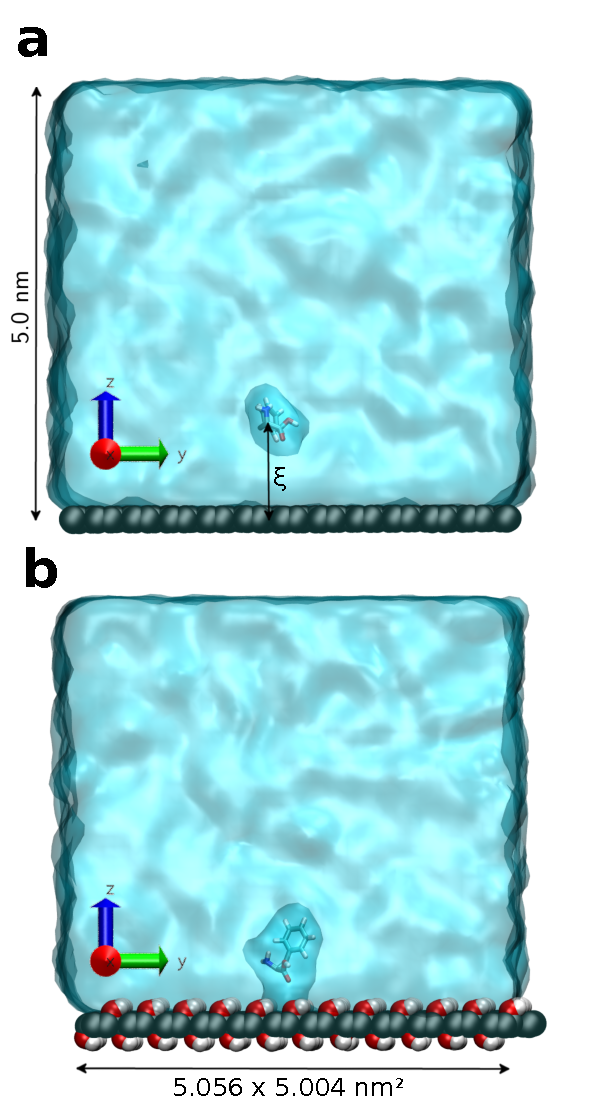
\includegraphics[width=.9\columnwidth]{Fig1.pdf}}
\caption[]{\label{fig:system-aminoacid} Example of simulated systems for single amino acids. (a) A phenylalanine  placed above a layer of pristine
  graphene inside a water-filled orthorombic box. (b) A phenylalanine molecule placed above a layer of partially oxidized graphene. Carbon atoms are depicted in gray whithin  the graphene layer, and cyan in the solute. Oxygen atoms and hydrogen atoms are depicted in red and white, respectively. $\xi$ is defined as the distance between the C$\alpha$ and the graphene layer projected along the $z$ axis.}
\end{figure}

\begin{figure}[htbp]
\centerline{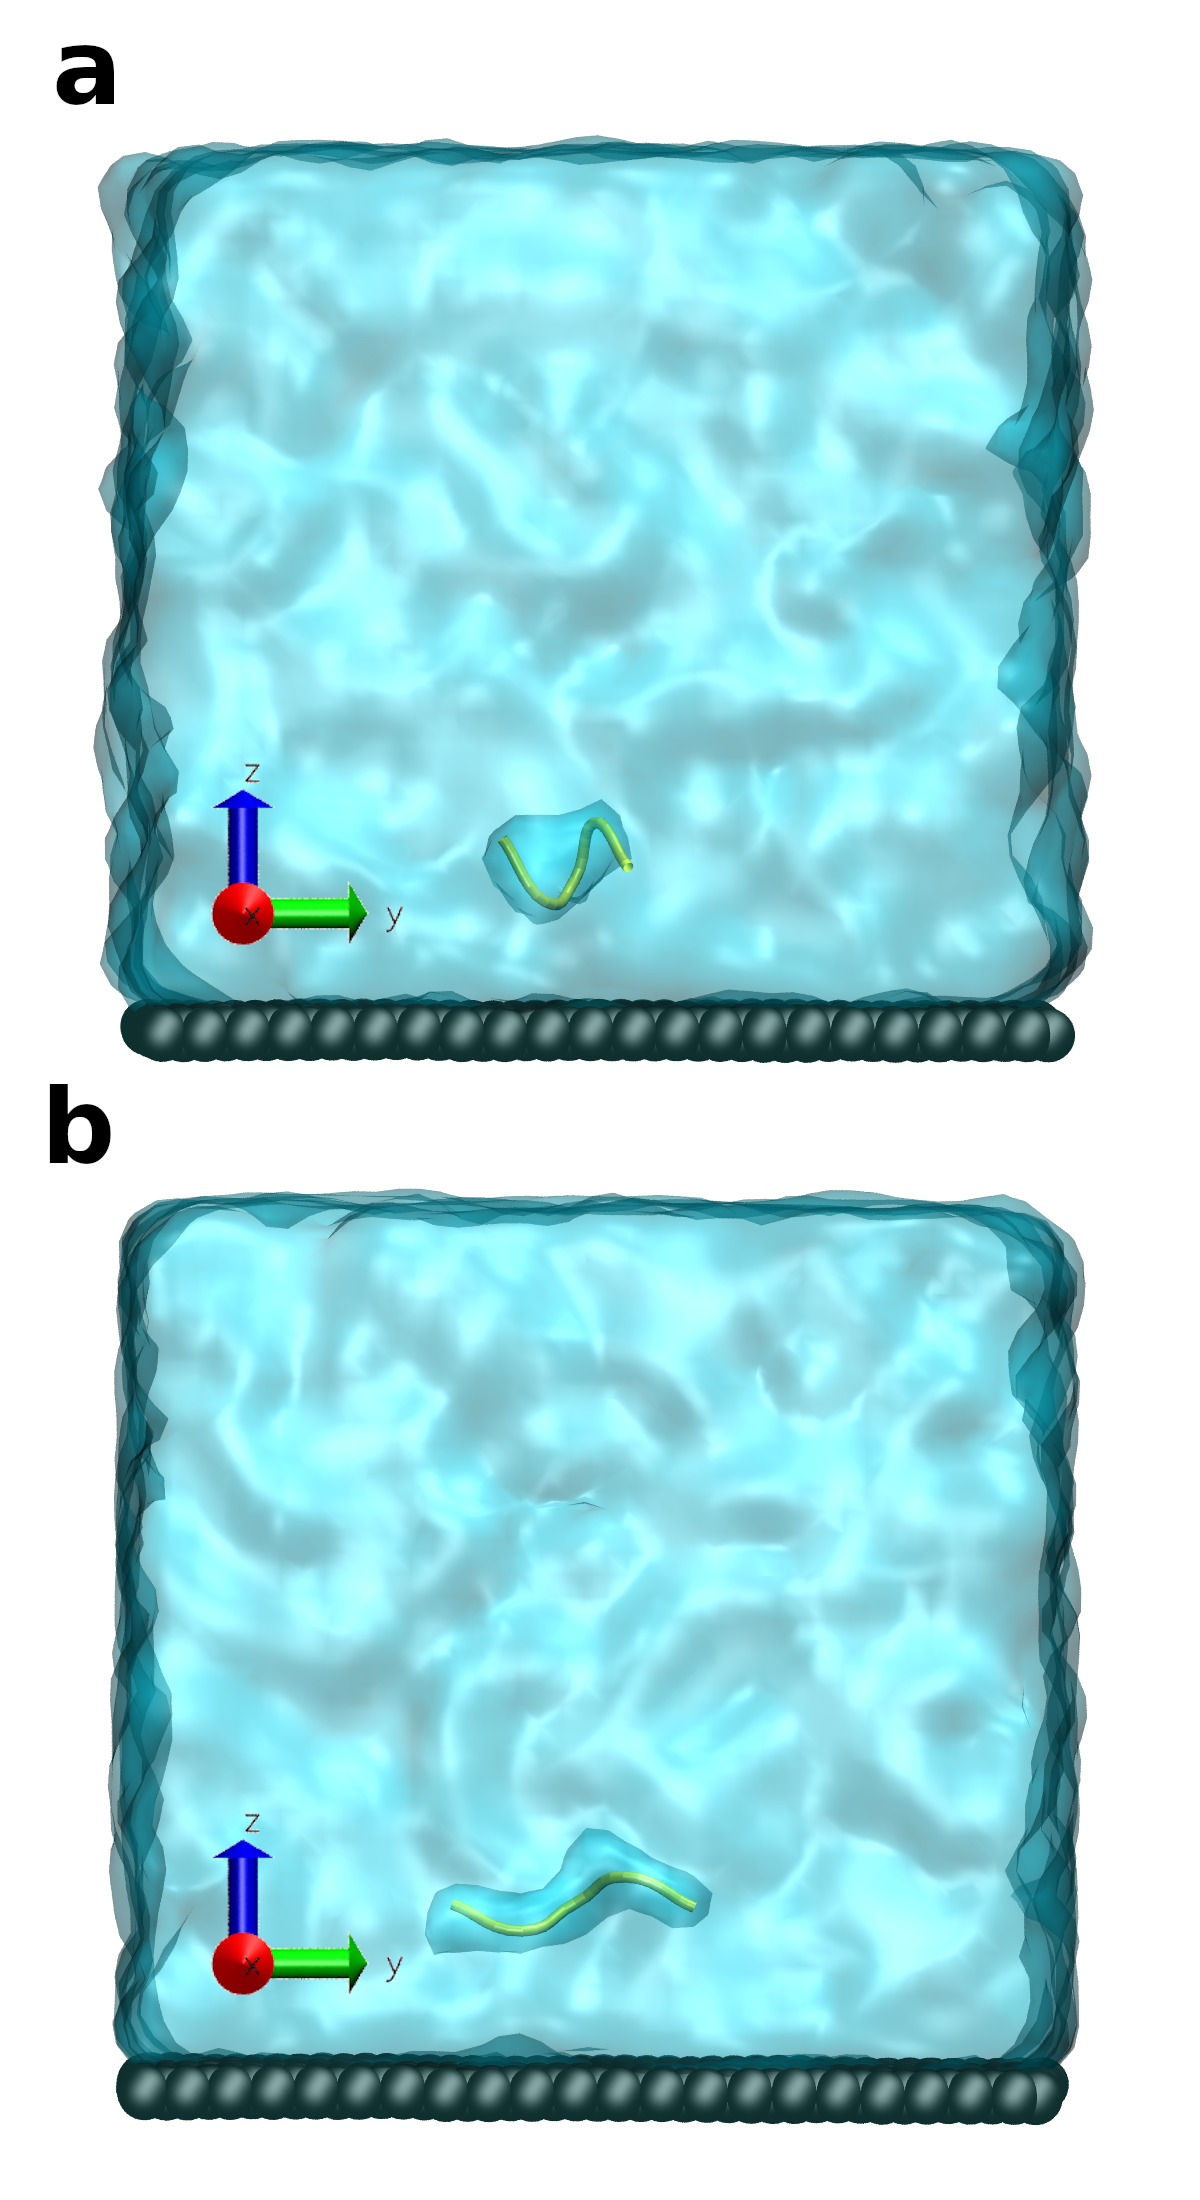
\includegraphics[width=.9\columnwidth]{Fig2.pdf}}
\caption[]{\label{fig:system-peptide} Simulated penta-L-alanine systems over pristine graphene. (a) Penta-L-alanine  in its $\alpha$-helical form; (b) Penta-L-alanine in its extended configuration. In both cases, harmonic distance restraints were used to keep the peptide in its respective configuration. Carbon atoms are depicted in gray. Penta-L-alanine molecules are depicted in yellow. $\xi$ is defined as the distance between the third C$\alpha$ and the graphene layer projected along the $z$ axis}
\end{figure}

\section{Results and discussion}

In this section we present the computed $\Delta A^{ads}$ for all 20 proteinogenic amino acids over pristine graphene.
We also investigate the energetic and entropic components of $\Delta A^{ads}$, paying attention to the different energy terms of the  $\Delta A^{ads}$.
We explore how these terms correlate with amino acid size and solvent exposure.
Additionally, we evaluate how partial oxidation of the graphene surface affects $\Delta A^{ads}$ for representative amino acids.
Finally, the possibility of employing the single amino-acids $\Delta A^{ads}$ to predict affinities of a penta-L-alanine peptide in its unfolded and $\alpha$-helical configurations towards graphene is evaluated.

\subsection{Adsorption free energy of amino acids over pristine graphene is correlated with size}

\begin{table}[htbp!]
\centering
\caption{\label{table:freeEnergy} Adsorption free energies ($\Delta A^{ads}0$), energies ($\Delta E^{ads}_{pot}$) and standard entropies ($T \Delta S^{ads}$)  in $[kJ \cdot mol^{-1}]$ for all amino acids (and a water molecule) over pristine graphene. The Side-chain charged state is denoted after the amino acid's name when relevant.}
\resizebox{\linewidth}{!}{%
\begin{tabular}{lrrr}
\toprule
%Name & $\Delta A^{ads}$ & $\Delta E^{ads}$ & $T \Delta S^{ads}$ \\ \hline
\multirow{2}{*}{Name}  & \multicolumn{1}{r}{$\Delta A^{ads}$} & \multicolumn{1}{r}{$\Delta E^{ads}_{pot}$ } & \multicolumn{1}{r}{$T \Delta S^{ads}$}  \\
\cline{2-4}            & \multicolumn{3}{c}{$[kJ \cdot mol^{-1}]$} \\ \hline
Alanine           & $-9.6  \pm 0.1$ & $-13.0 \pm 1.6$  & $-3.4  \pm 1.6$  \\
Arginine          & $-20.7 \pm 0.0$ & $-42.4 \pm 3.4$  & $-21.7 \pm 3.4$  \\
Arginine (+)      & $-18.5 \pm 0.0$ & $-53.3 \pm 5.8$  & $-34.8 \pm 5.8$  \\
Asparagine        & $-13.9 \pm 0.0$ & $-24.8 \pm 1.8$  & $-10.9 \pm 1.8$  \\
Aspartate (-) & $-9.5  \pm 0.0$ & $-11.0 \pm 1.6$  & $-1.5  \pm 1.6$  \\
Aspartic Acid     & $-15.9 \pm 0.0$ & $-25.9 \pm 2.1$  & $-10.0 \pm 2.1$  \\
Cysteine          & $-13.3 \pm 0.0$ & $-16.5 \pm 1.7$  & $-3.2  \pm 1.7$  \\
Glutamate (-) & $-7.5  \pm 0.0$ & $-6.3  \pm 1.5$  & $1.2   \pm 1.5$  \\
Glutamic Acid     & $-17.2 \pm 0.0$ & $-28.3 \pm 3.1$  & $-11.1 \pm 3.1$  \\
Glutamine         & $-16.4 \pm 0.0$ & $-24.1 \pm 1.5$  & $-7.6  \pm 1.5$  \\
Glycine           & $-8.0  \pm 0.0$ & $-16.2 \pm 1.4$  & $-8.3  \pm 1.4$  \\
Histidine (+)     & $-12.3 \pm 0.1$ & $-39.5 \pm 1.6$  & $-27.2 \pm 1.6$  \\
Histidine         & $-18.2 \pm 0.0$ & $-25.5 \pm 1.4$  & $-7.2  \pm 1.4$  \\
Isoleucine        & $-14.3 \pm 0.1$ & $-16.4 \pm 1.5$  & $-2.1  \pm 1.5$  \\
Leucine           & $-15.3 \pm 0.0$ & $-18.3 \pm 1.9$  & $-3.1  \pm 1.9$  \\
Lysine            & $-17.7 \pm 0.0$ & $-24.9 \pm 2.6$  & $-7.1  \pm 2.6$  \\
Lysine (+)        & $-11.4 \pm 0.1$ & $-27.4 \pm 1.6$  & $-16.0 \pm 1.6$  \\
Methionine        & $-19.4 \pm 0.0$ & $-38.3 \pm 6.2$  & $-18.9 \pm 6.2$  \\
Phenylalanine     & $-18.4 \pm 0.1$ & $-27.2 \pm 1.6$  & $-8.8  \pm 1.6$  \\
Proline           & $-6.0  \pm 0.0$ & $-24.1 \pm 1.5$  & $-18.1 \pm 1.5$  \\
Serine            & $-11.2 \pm 0.0$ & $-16.4 \pm 1.6$  & $-5.2  \pm 1.6$  \\
Threonine         & $-13.0 \pm 0.0$ & $-16.7 \pm 1.6$  & $-3.6  \pm 1.6$  \\
Tryptophan        & $-26.2 \pm 0.0$ & $-33.2 \pm 1.4$  & $-7.1  \pm 1.4$  \\
Tyrosine          & $-27.5 \pm 0.0$ & $-30.7 \pm 1.6$  & $-3.2  \pm 1.6$  \\
Valine            & $-12.6 \pm 0.0$ & $-11.5 \pm 1.6$  & $1.1   \pm 1.6$  \\
Water             & $3.3   \pm 0.1$ & $-3.6  \pm 2.8$  & $-6.9  \pm 2.8$  \\
\bottomrule
\end{tabular}
}
\end{table}

In the second column of Table \ref{table:freeEnergy} we present the $\Delta A_{ads}^0$ from the aqueous phase for all 20 proteinogenic amino-acids (and water) over pristine graphene computed via eq.\ref{eq:Adsorption}; the PMF profiles obtained via umbrella sampling are shown in Fig.S1. For Arg, Lys, His, Glu, and Asp, their side-chains in the neutral and charged states were computed as well.

All amino acids, not withstanding their chemical nature, present favorable $\Delta A^{ads}$ towards pristine graphene. This is in line with previous works by \citet{Dasetty2019} in which they tested several other force-fields, but their values are consistently deeper when compared to the ones reported in Table \ref{table:freeEnergy}.
Comparing free-energies require standard state corrections, as the volume for the unbound states may differ; thus  we corrected all $\Delta A^{ads}$ values  via eq. \eqref{eq:Standard}, which are shown in Figs. S10a and S10b. Notwithstanding, the differences with the values reported by \citet{Dasetty2019} still remain.

In this previous study all amino-acids were capped with acetyl and n-methyl amide groups \cite{Dasetty2019}, while in our case we just employed the uncharged N-terminal and C-terminal (NH$_2$ and COOH, respectively).
Consequently and to isolate the effects of the side-chains, in Fig. \ref{fig:AadsCorre}A we present the $\Delta A^{ads}$ reduced by the $\Delta A^{ads}$ of Gly.
When these reduced values are then compared our values exhibit a similar trend) and converge with previously repor ted data.\cite{Dasetty2019}
This comparison is displayed in Fig.S10 of the supplementary material, where the data shown in Fig.3b of \citet{Dasetty2019} is presented along with that of Fig.\ref{fig:AadsCorre}A of this study.

\begin{figure}[htbp]
\centerline{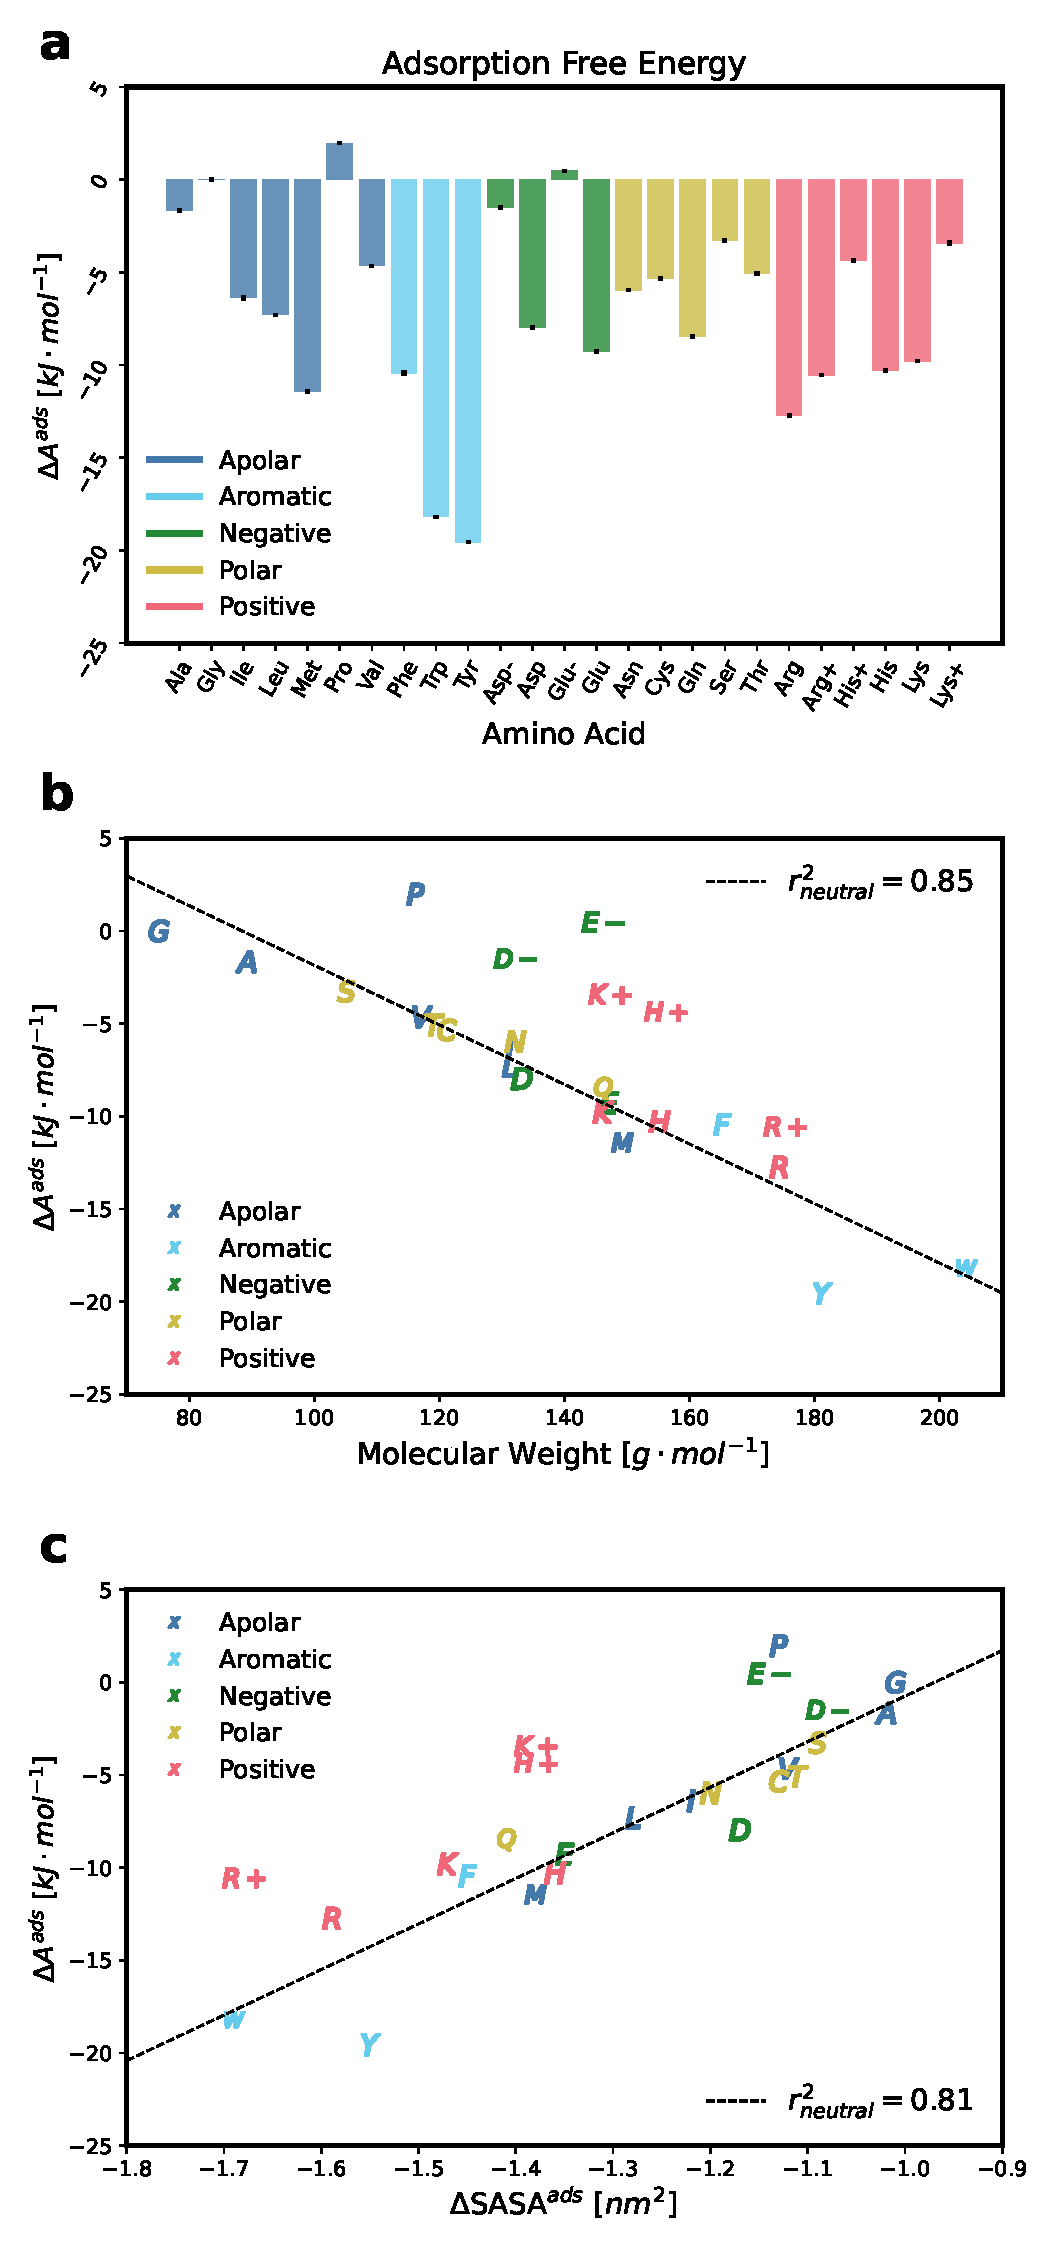
\includegraphics[width=.95\columnwidth]{Fig3.pdf}}
\caption[]{\label{fig:AadsCorre} Reduced adsorption free energies (i.e. with $\Delta A^{ads}$ of Gly set to $0$) for all amino acids. Unless otherwise noted, amino acids are in their neutral state. Charged species are indicated with a $+$ or $-$. (a) Reduced free energies ordered by the side-chain nature;  apolar (blue), aromatic (cyan), negative (green), polar (yellow), and positive (red). (b) $\Delta A^{ads}$ as a function of the molecular weight. (c) $\Delta A^{ads}$ as a function of $\Delta \textrm{SASA}^{ads}$. In (b) and (c) a linear regression is shown with a dotted line, and its respective $r^2$ value. This linear regression does not include amino acids in their charged state.}
\end{figure}

In detail, residues with aromatic groups, \emph{i.e.} Tyr, Trp, Phe, and His, are the strongest binders along with Arg and Met, which is consistent with cyclic voltametry and photoluminesence experiments.\cite{Mallineni_2016}
Arg+, despite its positive charge, has been previously found to strongly interact with graphene via density functional theory (DFT) calculations \cite{Tavassoli_2015, Singla_2016, Zhiani_2017} and MD studies.\cite{Pandey_2012, Dragneva_2013}
As expected, the neutral versions of Arg, Lys, His, Asp, and Glu, present deeper affinities when compared to their charged counterparts.
Gly, Pro, and Glu are the only residues  in which their sidechains reduce their affinity towards graphene.
Given that aromatic amino acids and Arg are among the ones that present the heaviest side chains.
This suggests a relation between size and $\Delta A^{ads}$.
Thus, in Fig.\ref{fig:AadsCorre}B we plotted the reduced $\Delta A^{ads}$ as function of their molecular weight.
There is a noticeable correlation between the molecular size and the binding strength; charged amino-acids, with the notable exception of Arg+, do not follow this trend and thus a linear regression considering only neutral amino acids is presented herein.
Apart from charged amino acids, Pro and Tyr are the only special cases that do not strictly follow this trend.
Nonetheless, the linear models show a strong correlation with an $r^2$ of 0.85 (the $r^2$ including charged amino acids is around 0.6).
As our graphene model only includes VdW interactions, this strong correlation suggests that the $\Delta A^{ads}$ is dominated by dispersion interactions between amino acids and graphene, as the later are proportional to the molecular size. Nonetheless, the water removal from the surface, the so called "hydrophobic effect" could also play an important role in the adsorbtion process.
To get a further physical insight, we explored whether this correlation was also present for the differences in the solvent-accessible surface area (SASA) between the adsorbed and unbound states.
The SASA of each amino acid was calculated using the algorithm of \citet{Lee_1971} for all simulated windows, then the difference between the near and free states ($\Delta\textrm{SASA}^{ads}$) was calculated using eqs. \ref{eq:WHAM-unbias} and \ref{eq:Eads}.
In this way, in Fig. \ref{fig:AadsCorre}C the reduced $\Delta A^{ads}$ are plotted as function of $\Delta\textrm{SASA}^{ads}$.
We observed a very similar correlation strength ($r^2=0.83$) when removing charged amino acids.
%It becomes interesting to explore this correlation in light of the amount of water removed upon amino acid adsorption.
Our interest in this correlation also arises from its relation to the amount of water removed upon amino acid adsorption.
The negative of $\Delta\textrm{SASA}^{ads}$ is a measurement of the effective interaction surface between the amino acid and graphene; from the volume of a water molecule ($V_w\sim0.03\textrm{nm}^3$) and assuming a perfect spherical geometry, the surface area of a single water molecule (SA$_w$) is close to 0.5 nm$^2$.
Trp being the heaviest amino acid, exhibits the largest interaction surface, which is approximately 4 times the SA$_w$; for Gly this is closer to 2 times SA$_w$.
Thus, the adsorption process approximately removes a range of 2 to 4 water molecules from the graphene surface.
One can, in a broad and linear manner, estimate the water removal contribution to the binding strength towards graphene by multiplying the number of removed water particles by the $\Delta A^{ads}$ of a single water molecule (see Table \ref{table:freeEnergy}).
For Trp this is around 60\% of the $\Delta A^{ads}$ reported in Table \ref{table:freeEnergy},  revealing the importance of the removal of interfacial water from the surface. The latter only considers the water-graphene interaction and does not include the desolvation of the amino-acid, (see section below for a deeper analysis on this topic) As the $\Delta\textrm{SASA}^{ads}$ provides a concrete physical interpretation, this descriptor will be employed for the rest of the correlation analyses.
In the next section, we explore in more detail the energetic (and entropic) contributions to the adsorption strength of each amino acid.

\subsection{The energy and entropy of adsorption exhibit a lower correlation degree with size}

In the third and fourth columns of Table \ref{table:freeEnergy}, the total adsorption potential energy and entropy towards graphene ($\Delta E_{pot}^{ads}$ and $T\Delta S^{ads}$, respectively) for each amino acid are presented; the energies and entropies reduced by the $\Delta E_{pot}^{ads}$ and $ T\Delta S^{ads}$ of Gly, respectively, are presented in Fig. \ref{fig:EneCorr}, as well.

\begin{figure}[htbp]
\centerline{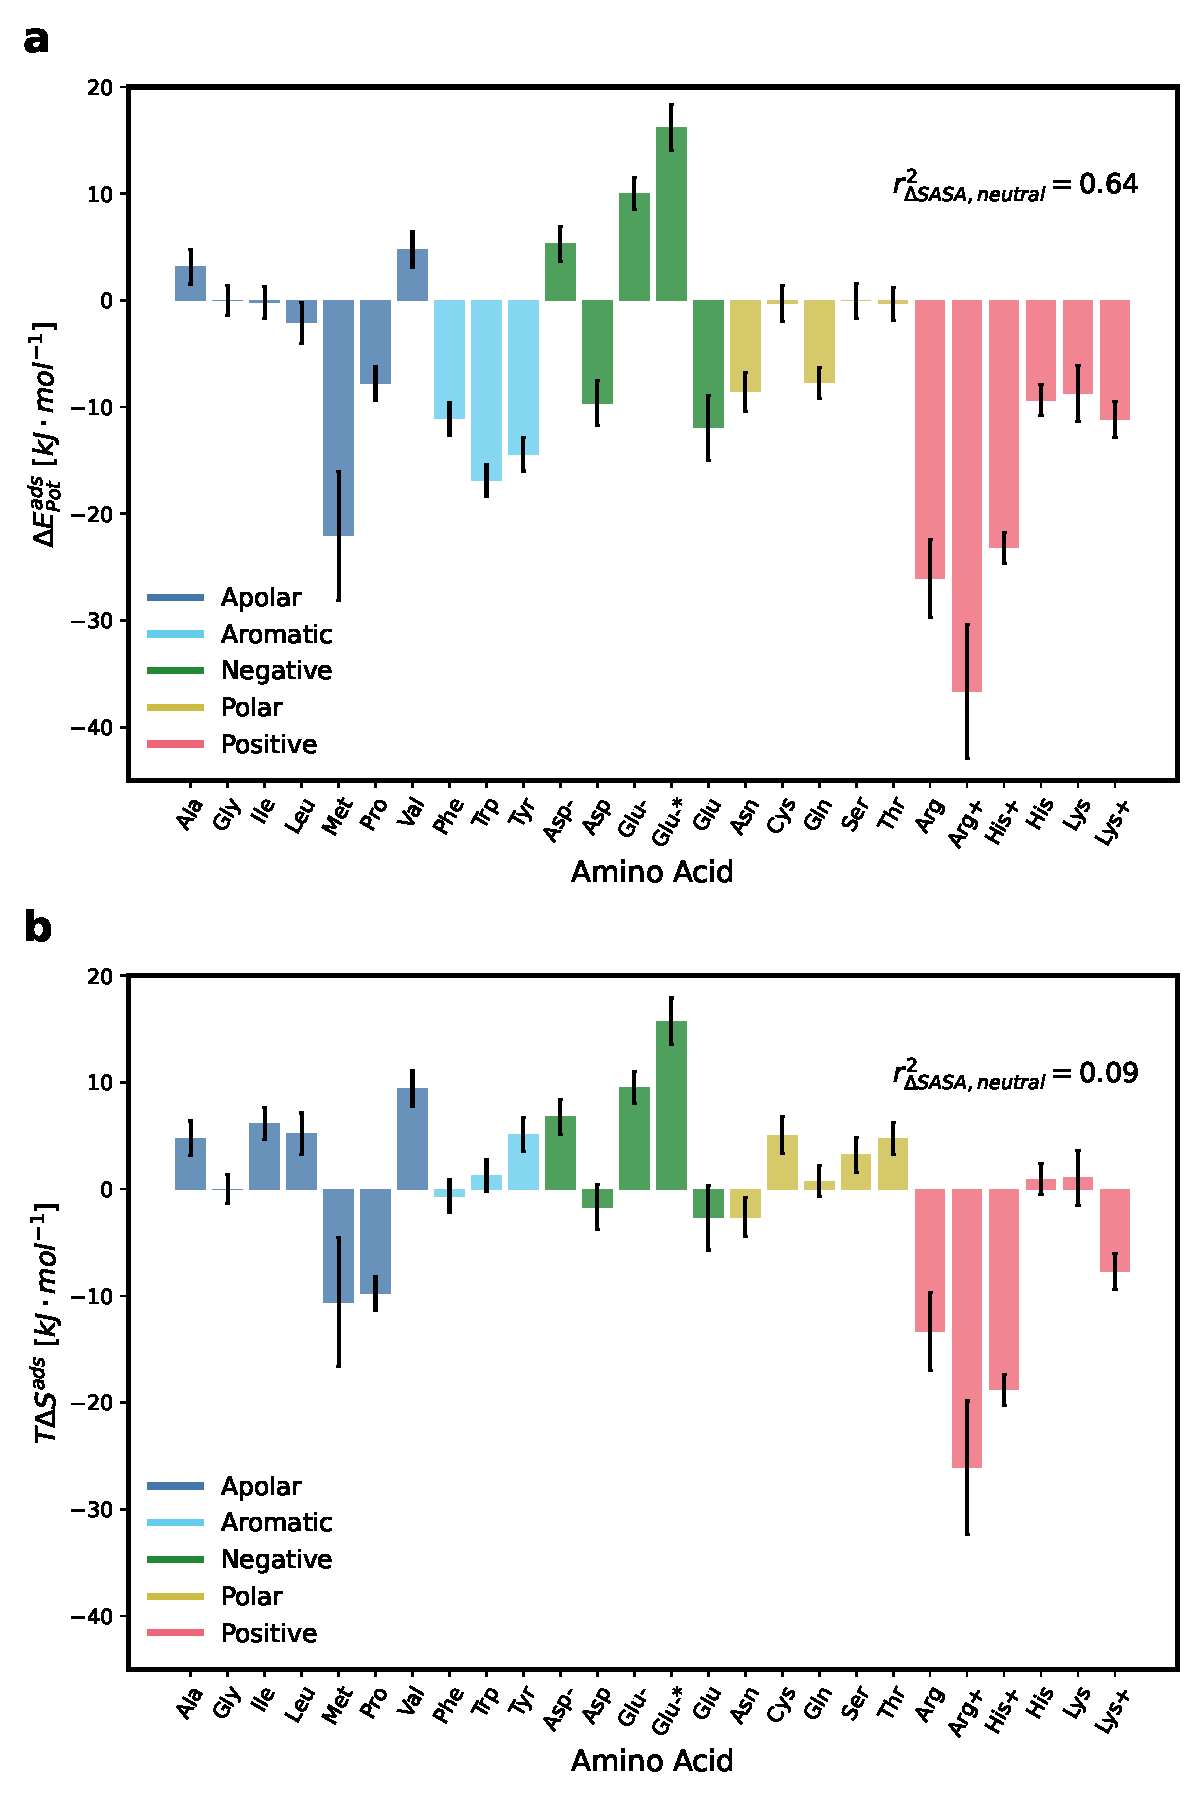
\includegraphics[width=\columnwidth]{figures/Fig4.pdf}}
\caption[]{\label{fig:EneCorr} Reduced total adsorption potential energies, $\Delta E_{pot}^{ads}$, (a) and entropies, $T\Delta S^{ads}$, (b) (b) for all amino acids. In both panels the correlation coefficient ($r^2$) is included, for the linear regression between $\Delta E_{pot}^{ads}$ and $ T\Delta S^{ads}$ against the $\Delta$SASA of adsorption for the neutral species.}
\end{figure}


All $\Delta E_{pot}^{ads}$ are negative and, in their majority, deeper than their respective $\Delta A^{ads}$.
The only exceptions to this trend are Glu- and Val.
However, these two values differ by less than their error estimates (which in turn are below thermal noise at 298 K) from their respective $\Delta A^{ads}$.
Therefore, the adsorption process is mainly energetically driven.
When evaluating the energetic contributions of each side-chain, the overall trend is to favor adsorption; only Asp-, Glu-, Ala, and Val, exhibit significantly higher values with respect to Gly (see Fig.\ref{fig:EneCorr}a).
Thus its not strange that still a correlation (when removing charged amino-acids) between $\Delta E^{ads}_{pot}$ and $\Delta \textrm{SASA}^{ads}$ exists, although weaker than the one observed for the $\Delta A^{ads}$ (see Figs. S9a and S9b).
Despite the apolar nature of the graphene layer, there is an asymmetry between positively and negatively charged amino acids; for the former, the charged versions present deeper $\Delta E_{pot}^{ads}$ than their neutral versions; for the latter, the opposite trend is present.
Quite interestingly, for His and Arg their $\Delta \textrm{SASA}^{ads}$ are lower for their charged versions (see Fig.\ref{fig:AadsCorre}); and in the opposite way for Glu and Asp these are higher for their charged counterparts; thus one again could explain these differences by the interaction surfaces between the amino acid and graphene. Another contributing factor to this difference are cation--$\pi$ interactions between the positively charged amino acids and graphene. Arg in particular has been observed to stack with aromatic molecules \cite{Flocco_1994}, explaining its strong energetic interactions.
In this aspect, His stands out for having a relatively weak $\Delta E^{\textrm{ads}}$, even though its aromatic nature should too result in $\pi-\pi$ stacking interactions.
To explore the latter, we estimated the prevalence of $\pi$-$\pi$, cation-$\pi$ and guanidinium-$\pi$ interactions for Arg, His, Tyr, Lys  which are shown in Table S3. In this regard, both positive Arg and His exhibit a 37\% and 8\% increment in their stacking interactions when compared to their neutral versions; thus in line with the deeper $\Delta E^{\textrm{ads}}$ for the charged Arg and His.
Moreover, the larger difference in the stacking interactions between Arg and His are in accordance with the $\Delta E^{\textrm{ads}}$ shown in Fig.\ref{fig:EneCorr}. Finally, all aromatic species present stacking percentages above 70\%; and these are the deeper binders towards graphene.

$T\Delta S^{\textrm{ads}}$ terms are in their majority negative (see fourth column of Table \ref{table:freeEnergy}), a typical example of the well known energy-entropy compensation.\cite{Liu2001,Leung2008,Chodera2013,Ryde2014,Fox2018}
Only Glu- and Val have positive values, and these are lower than their respective error margins and  thermal noise \textit{i.e.}, these differences are close to entropy neutral.
Reducing the values by Gly (see Fig.\ref{fig:EneCorr}b) shows both positive and negative side-chain contributions to the entropy.
This is reflected in a low correlation with $\Delta$SASA ($r^2= 0.09$).



\subsection{The adsorption mechanism is dominated by dispersion and water-water interactions and is preceded by a desolvation and a dewetting process}

To attain a deeper understanding of the adsorption process,  we decomposed the reduced $\Delta E^{ads}_{pot}$ into the interacting pairs involving the solute: aminoacid-graphene ($\Delta E^{ads}_{AA-Graph}$) and aminoacid-water ($\Delta E^{ads}_{AA-H_2O}$) pairs  which are presented in Fig.\ref{fig:EneAACorr}; and the pairs involving the solvent: water-graphene ($\Delta E^{ads}_{H_2O-Graph}$) and water-water ($\Delta E^{ads}_{H_2O-H_2O}$) shown in fig.\ref{fig:EneH2OCorr}. All these energetic terms were computed via  Eqs.~\ref{eq:WHAM-unbias}. Furthermore, we present the raw energy differences (i.e., before reducing the values to set Gly to 0) in Table~S1.

\begin{figure}[htbp]
\centerline{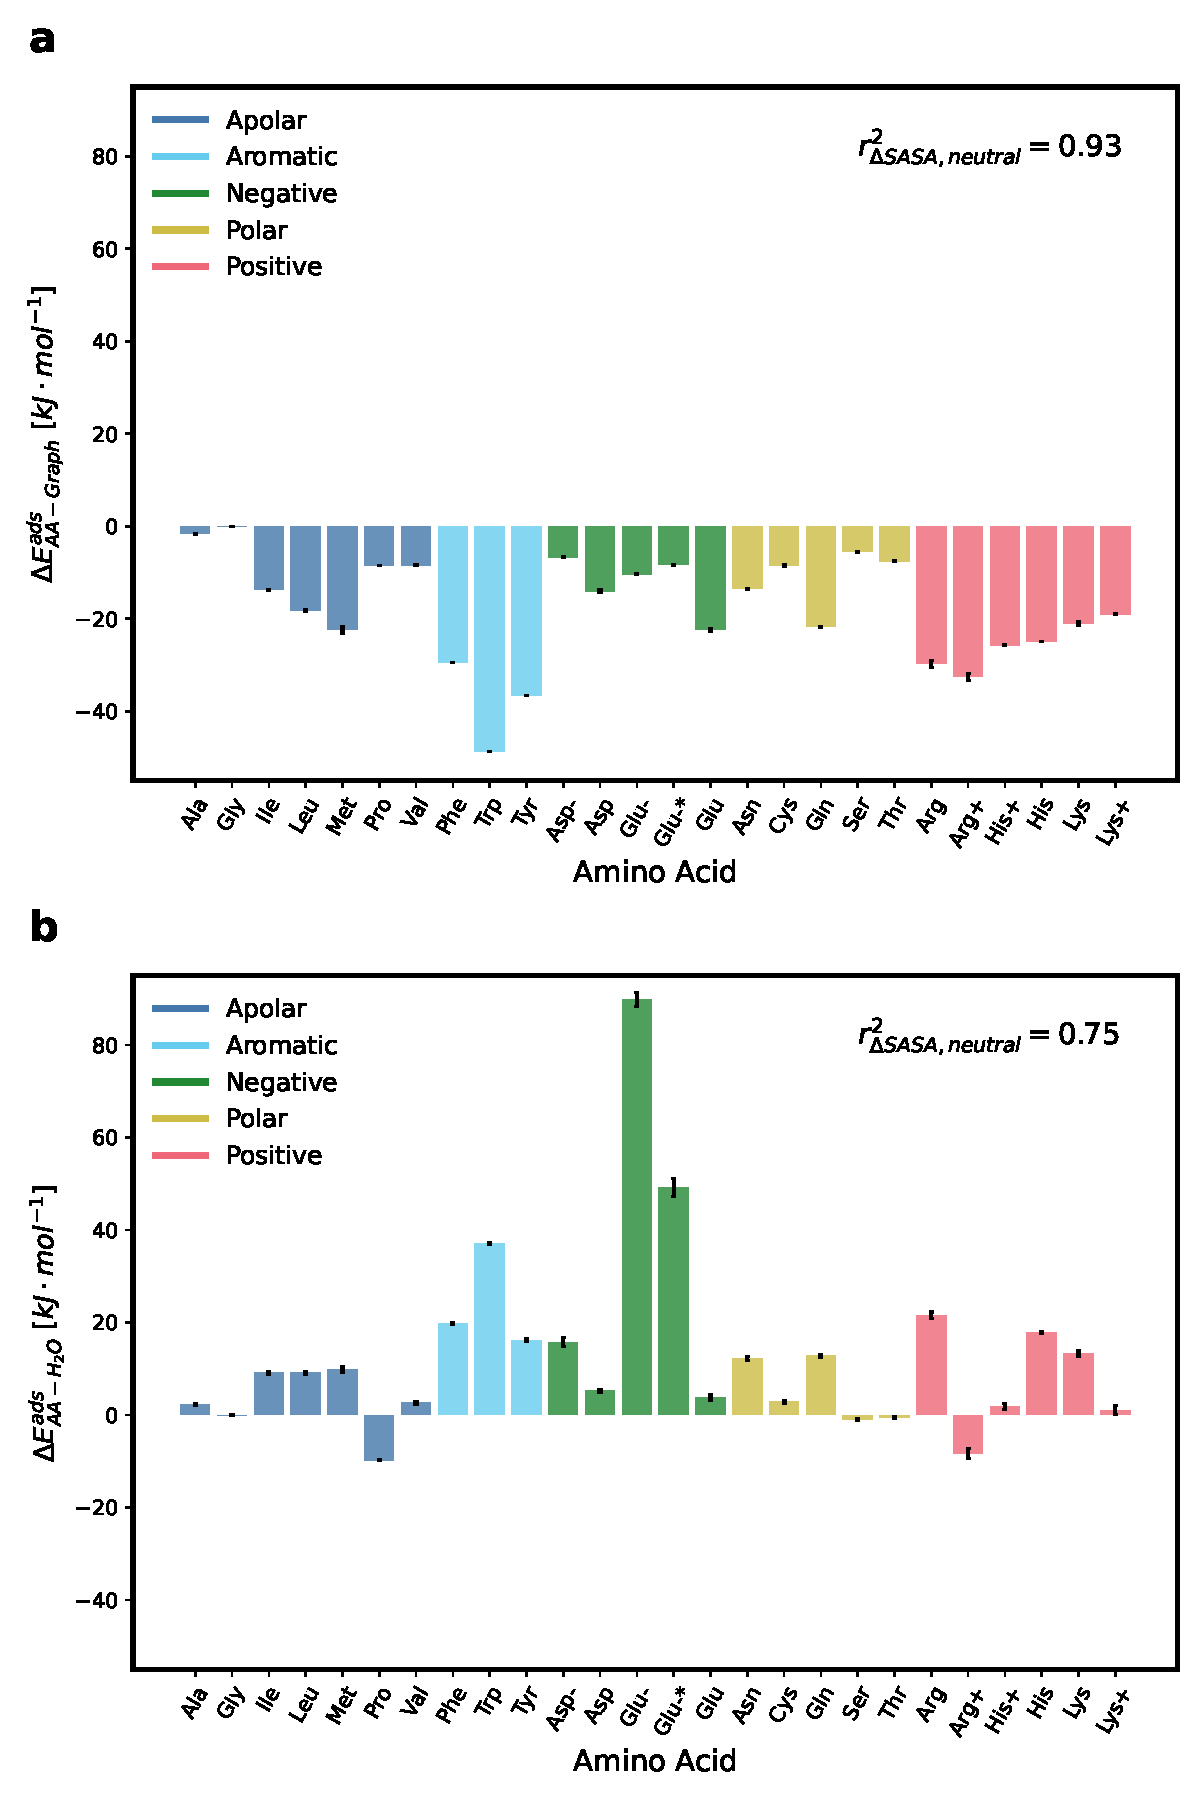
\includegraphics[width=\columnwidth]{figures/Fig5.pdf}}
\caption[]{\label{fig:EneAACorr} Reduced solute adsorption interaction energies with graphene (a) or water (b) for all amino acids. In both panels a correlation coefficient is included, which describes a linear regression between the presented energy component against the $\Delta$SASA of adsorption of the amino acids simulated in their \textit{neutral} state. Ordering, coloring, and notation for both panels follow the conventions used in Fig.~\ref{fig:AadsCorre}a.}
\end{figure}

\begin{figure}[htbp]
\centerline{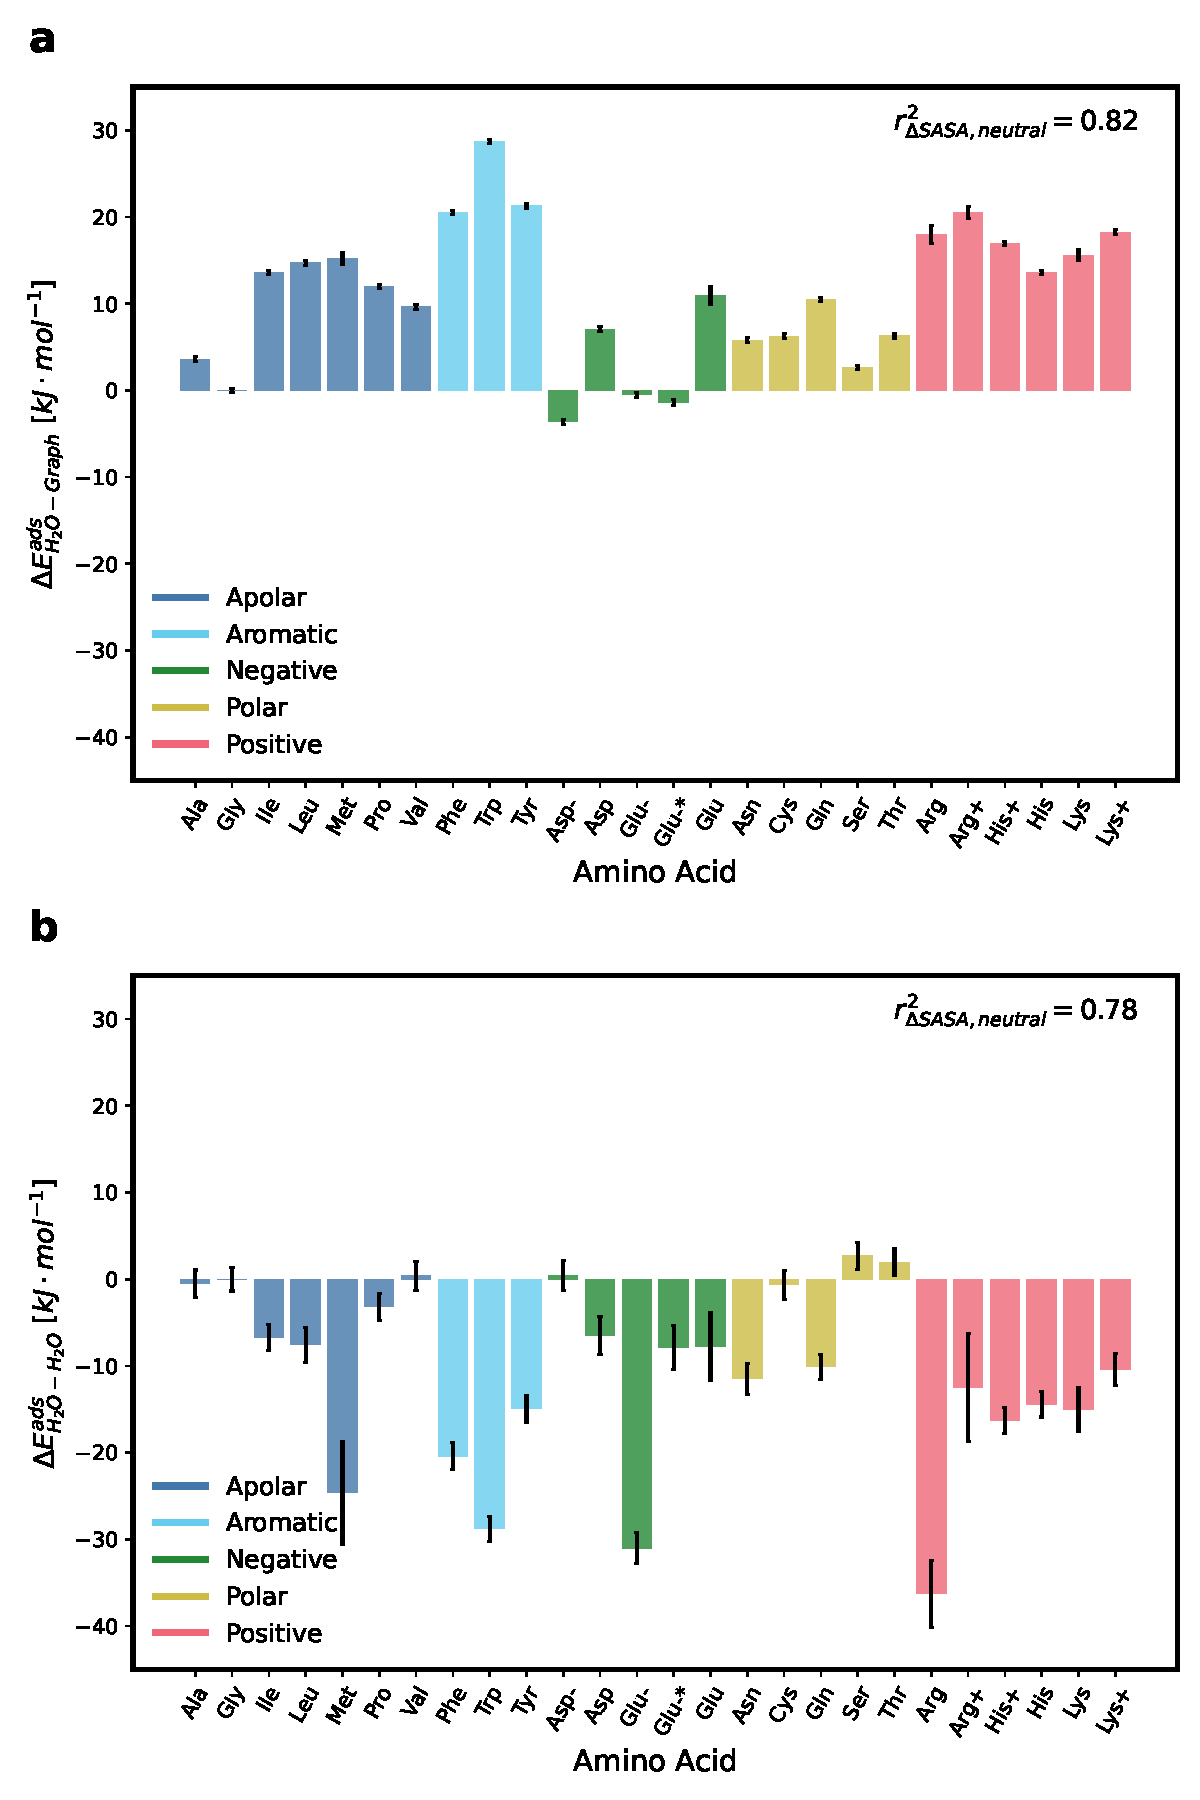
\includegraphics[width=\columnwidth]{figures/Fig6.pdf}}
\caption[]{\label{fig:EneH2OCorr}Reduced solvent adsorption interaction energies with graphene (a) or water (b) for all amino acids. In both panels a correlation coefficient is included, which describes a linear regression between the energy or entropy against the $\Delta$SASA of adsorption of the amino acids simulated in their \textit{neutral} state. Ordering, coloring, and notation for both panels follow the conventions used in Fig.~\ref{fig:AadsCorre}a.}
\end{figure}

All $\Delta E^{ads}_{AA-Graph}$ and $\Delta E^{ads}_{H_2O-H_2O}$ terms favor adsorption an are similar in magnitude thus revealing the importance of the hydrophobic effect which means that water interacts more favourably with itself than with the partners; all $\Delta E^{ads}_{H_2O-Graph}$ and $\Delta E^{ads}_{AA-H_2O}$ terms favor removal of the amino acid from the graphene surface.
To obtain a more detailed description,in figures S4 through S7, we provide  the individual profiles of these energies as a function of the reaction coordinate ($\xi$) for all amino acids and water.
In detail, the adsorption process involves: i) an increase in the $E^{ads}_{AA-Graph}$ interactions (see Fig.S4) with very smooth profiles and a single minimum without any barriers and a very steep slope appearing around $\xi=0.7$; some residues present a two-stage adsorption process with a sigmoidal profile within intermediate stages (Leu, Phe, Tyr, and Arg); ii) a decrease in the $E^{ads}_{AA-H_2O}$ interaction (see Fig. S5) which represents the desolvation process which appears around $\xi=1.0~nm$,  in general, these profiles present several minima along the adsorbtion pathway; we have found that these are related to the formation of intramolecular interactions within the aminoacids that reduce the interactions with water but as a whole they cancel out; iii) a reduction of of the $E^{ads}_{H_2O-Graph}$ interactions (see Fig.S6), in other words the dewetting of the surface, the latter becomes relevant at $\xi \sim 0.9 nm $ and iv) an increase in $E^{ads}_{H_2O-H_2O}$ interactions (see Fig. S7), with a noticeable change in the slope around $\xi \sim 0.6 nm $. Overall, these profiles reveal that the desolvation of the aminoacid and the dewetting of the graphene surface are events that precede adsorption.

The fact that there is practical no difference between the molecular weight and $\Delta$SASA is an indication that no relevant conformational changes are present upon adsorption, which is expected due to relatively small size of the studied chemical species. To confirm the latter, we also computed the changes in the intramolecular energies upon adsorption ($\Delta E^{intra}$), shown in fig. S8. In general, the $\Delta E^{intra}$ are close to $k_{B}T$ even though along the adsorption pathway there are several maxima and minima. Quite interestingly, these valleys and hills cancel out with the  $E^{ads}_{AA-H_2O}$ terms (see Fig. S5). An extreme case of the aforementioned term cancellation involves Glu- in which the $\Delta E^{intra}$ becomes substantially favorable upon adsorption (see Fig. S8):  This was the result of the formation of an internal H-bond between the side-chain carboxilic group and both c and n terminals upon adsorbtion. Consequently the $\Delta E^{ads}_{AA-H_2O}$ and the $\Delta E^{ads}_{H_2O-H_2O}$ become substatianlly unfavourable and favourable, respectively.  In fact, we recomputed these pair interactions by including only the configurations in which this intramolecular interaction was absent (see Glu-$^*$ in Figs. \ref{fig:EneCorr}-\ref{fig:EneH2OCorr})and as expected  the $\Delta E^{ads}_{AA-H_2O}$ and the $\Delta E^{ads}_{AA-H_2O}$ are reduced and increased, respectively and much more in line with the rest of the aminoacids. Quite interestingly, the formation of this intramolecular interactions do not affect the  $\Delta E^{ads}_{AA-Graph}$ and $\Delta E^{ads}_{H_2O-Graph}$.
In the context of protein adsorption, these intramolecular interactions will not be present.
%Thus it is important to asses the impact of the intramolecular interactions on the affinity towards graphene, which do not directly affect the interaction with graphene and are cancelled by a reduction of interactions with solvent and an increase in the solvent-solvent interactions.
Nonetheless, to avoid these minor issues, capping the terminals of peptides with non-polar groups is suggested, specially for polar and charged residues.


From the values presented in Table S1 we can explore the energy terms involving the amino acids (this is the sum of the the second and third columns of Table S1; $\Delta E^{ads}_{AA-Graph, AA-H_2O}$) in contrast to the rest of the terms (the sum of the fourth and fifth columns; $\Delta E^{ads}_{H_2O-Graph, H_2O-H_2O}$) are the dominant forces for the adsorption process (see Table S2).
In this regard, all $\Delta E^{ads}_{AA-Graph, AA-H_2O}$  are favorable; 77\% (20 residues) of all amino acids exhibit a $\Delta A^{ads}-\Delta E^{ads}_{AA-Graph, AA-H_2O} \leq 3k_BT$ (see 4th column of Table S3) with 7 an 9 amino acids  having a $\Delta A^{ads}-\Delta E^{ads}_{AA-Graph, AA-H_2O}$ below 1 and 2 $k_BT$, respectively.
Thus, for the majority of the amino acids, the $\Delta E^{ads}_{AA-Graph, AA-H_2O}$ and $\Delta A^{ads}$ do not differ, on average, by more than 20\%.
Consequently, for this group, the adsorption process is clearly dominated by the graphene-aminoacid interaction.
On the other hand, there is a group of 7 amino acids in which $\Delta E^{ads}_{AA-Graph, AA-H_2O}$ substantially differs from $\Delta A^{ads}$.
In this case, the $\Delta E^{ads}_{AA-Graph, AA-H_2O}$ are much deeper than their respective $\Delta A^{ads}$ (with the only exception of Asp-).
These residues are the positively charged ones and Proline.
And, as shown in figs. \ref{fig:AadsCorre}b and \ref{fig:AadsCorre}c, these are the outliers from the linear regressions.
In line with the above mentioned, the $\Delta E^{ads}_{H_2O-Graph, H_2O-H_2O}$ terms in their vast majority are close to $k_BT$, thus the water removal from the surface, in terms of its energetic contribution is only relevant for few residues such as Arg, Glu- and Met.

As a whole, the dominant term to the adsorption towards graphene is the favorable interaction between the amino acid and  graphene and kinetically the adsorption is preceded by a simultaneous dewetting and desolvation process. This is true even for the charged amino acids, despite the graphene model being completely charge-neutral. The relative magnitude of the $\Delta E^{ads}_{AA-Graph}$ is in agreement, in particular for the most and least favorable amino acids, with the results reported by \citet{Pandey_2012} for amino acids in a peptide chain. Moreover, our results are in line with those reported for capped amino acids rather than uncapped zwitterionic amino acids.\cite{Dragneva_2013}
That is to say, our results are indicative of uncapped non-zwitterionic amino acids and therefore a representative  model for side-chain properties in peptide chains.



\subsection{Partial graphene oxidation recovers affinity by chemical nature}

Our previous results, in a general manner, indicate that the amino acid chemical nature --\emph{i.e.} polarity, charge or hydrophobicity-- is not critically relevant for the adsorption process towards graphene.
This is line with many reports that demonstrate that graphene strongly interacts with proteins and other biological macromolecules.\cite{Zhang2013,Chong2015,Puigpelat_2019,Duan_2015,Zhou2014,Lalwani_2016}
Consequently, graphene oxide (GO) has been proposed to reduce these strong interactions and has been proposed as a biocompatible material for many applications.\cite{Gomez-Navarro2010,Rhazouani2021}
In this way, we carried out PMF calculations for a subset of amino acids (and water) over GO (25\% of oxidation); these species were chosen to include one sample of each of the following side-chain groups: positive, negative, polar, apolar, and aromatic.
The PMF profiles are presented in Fig. S4.
For these selected amino acids, Table~\ref{table:freeEnergyOxidized} compares the $\Delta A^{ads}$ over pristine graphene (using the same data from Table~\ref{table:freeEnergy}, now labeled as $\Delta A^{ads}_{Graph}$) with the free energy of adsorption over our oxidized graphene model ($\Delta A^{ads}_{GO}$), as shown in Fig~\ref{fig:system-aminoacid}b.

As shown in Table~\ref{table:freeEnergyOxidized}, adsorption over GO is notably less favorable than over pristine graphene.
Moreover, the chemical nature of the aminoacid now serves to explain these results.
In particular, Phe adsorption turns unfavorable while Ile adsorption is close to free-energy neutral at only $0.1 \pm 0.1 [kJ\cdot mol^{-1}]$.
A drastic change in Phe was expected as $\pi-\pi$ stacking capabilities have been shown in an MD and DFT study to be the principal predictor of adsorption of aromatic compounds onto GO.\cite{Tang_2018}
These changes indicate that the graphene adsorption properties are sensible to even relatively small changes to the surface; at 25\% oxidation its distribution over both faces of the layer results in the surface of adsorption only presenting one oxygen atom for every 8 carbon atoms.
The general closeness of $\Delta A^{ads}_{GO}$ to 0 $[kJ \cdot mol^{-1}]$ suggests that even this proportion is enough to make the surface similar to the solvent with regards to adsorption from the aqueous solution.
This is consistent with descriptions of GO as a much more hydrophilic material than graphene; physical and \textit{in silico} experiments have shown that GO adsorbs water at higher rates than typical hygroscopic materials like silica gel.\cite{Lian_2018}



\begin{table}[htbp]
\centering
\caption{\label{table:freeEnergyOxidized} Comparison of adsorption free energies over pristine graphene ($\Delta A^{ads}_{Graph}$) and over oxidized graphene ($\Delta A^{ads}_{GO}$) for a selection of amino acids (and a water molecule). Charged state is denoted after the amino acid's name where relevant; otherwise the amino acid was simulated in its neutral state.}
\resizebox{\linewidth}{!}{%
\begin{tabular}{lrr}
\toprule
%Name & $\Delta A^{ads}_{Graph}$ & $\Delta A^{ads}_{GO}$ \\ \hline
\multirow{2}{*}{Name}  & \multicolumn{1}{r}{$\Delta A^{ads}_{Graph}$} & \multicolumn{1}{r}{$\Delta A^{ads}_{GO}$}  \\
\cline{2-3}            & \multicolumn{2}{c}{$[kJ \cdot mol^{-1}]$} \\ \hline
Arginine (+)      & $-18.5 \pm 0.0$ & $-1.6 \pm 0.1$    \\
Asparagine        & $-13.9 \pm 0.0$ & $-3.4 \pm 0.1$    \\
Glutamic Acid (-) & $-7.5  \pm 0.0$ & $-1.9 \pm 0.1$    \\
Glycine           & $-8.0  \pm 0.0$ & $-1.8 \pm 0.1$    \\
Isoleucine        & $-14.3 \pm 0.1$ & $0.1  \pm 0.1$    \\
Phenylalanine     & $-18.4 \pm 0.1$ & $1.7  \pm 0.1$    \\
Water             & $3.3   \pm 0.1$ & $2.0  \pm 0.1$    \\
\bottomrule
\end{tabular}
}
\end{table}


%%% Old: dA, dE, TdS
% \begin{table}
% \centering
% \caption{\label{table:freeEnergyOxidized} Adsorption free energies ($\Del% ta A^{ads}$), energies ($\Delta E^{ads}$), and entropies($T \Delta S^{ads% }$) for a selection of amino acids (and a water molecule) over oxidized g% raphene. Charged state is denoted after the amino acid's name where relev% ant; otherwise the amino acid was simulated in its neutral state.}
% \resizebox{\linewidth}{!}{%
% \begin{tabular}{lrrr}
% \toprule
% Name & $\Delta A^{ads}$ & $\Delta E^{ads}$ & $T \Delta S^{ads}$ \\ \hline
% Arginine (+)      & $-1.6 \pm 0.1$ & $-4.1  \pm 2.7$  & $-2.5  \pm 2.7$  % \\
% Asparagine        & $-3.4 \pm 0.1$ & $-12.0 \pm 2.8$  & $-8.6  \pm 2.8$  % \\
% Glutamic Acid (-) & $-1.9 \pm 0.1$ & $-8.5  \pm 2.9$  & $-6.5  \pm 2.9$  % \\
% Glycine           & $-1.8 \pm 0.1$ & $-1.1  \pm 2.8$  & $0.8   \pm 2.8$  % \\
% Isoleucine        & $0.1  \pm 0.1$ & $0.4   \pm 3.0$  & $0.4   \pm 3.0$  % \\
% Phenylalanine     & $1.7  \pm 0.1$ & $-13.7 \pm 2.9$  & $-15.3 \pm 2.9$  % \\
% Water             & $2.0  \pm 0.1$ & $-2.8  \pm 4.9$  & $-4.8  \pm 4.9$  % \\
% \bottomrule
% \end{tabular}
% }
% \end{table}

\subsection{The single amino acid $\Delta A^{ads}$ can serve to predict adsorption of larger peptides.}

The correlation between adsorption affinity and $\Delta \textrm{SASA}^{ads}$ naturally leads to the following question: can we employ the single amino-acids $\Delta A^{ads}$ to predict the $\Delta A^{ads}$ of larger peptides?
In other words, is it possible to employ the linear model shown in Fig. \ref{fig:AadsCorre}C to estimate the $\Delta A^{ads}$ towards graphene of larger molecules?
To do so, we rigorously computed the $\Delta A^{ads}$ of a penta-L-alanine peptide  in two different configurations: helical and stretched, as shown in Fig.~\ref{fig:system-peptide} panels a and b, respectively.
Then, we estimated $\Delta A^{ads}$ by only computing  $\Delta \textrm{SASA}^{ads}$ and employing the linear regression of Fig. \ref{fig:AadsCorre}C (to avoid over fitting we removed Ala from the regression); the rationale behind choosing both penta-L-alanine configurations is to check whether our model is capable of differentiating between cases of different $\Delta \textrm{SASA}^{ads}$ for the same molecule.
Accordingly, in Fig.S3 and Table \ref{table:predictions} the PMF profiles and computed $\Delta A^{ads}$  for both penta-L-alanine configurations are presented, respectively.
Table~\ref{table:predictions} also includes the computed $\Delta \textrm{SASA}^{ads}$ (third column) and predicted $\Delta A^{ads}$ for alanine, penta-L-alanine (Helix), and penta-L-alanine (stretched); for both the $\Delta \textrm{SASA}^{ads}$ (PV$_{\textrm{SASA}}$) and the molecular weight (PV$_{\textrm{MW}}$)) models (see Figs. \ref{fig:AadsCorre}B and C), which are shown in the fifth and sixth columns of Table ~\ref{table:predictions}.


 \begin{table*}[htbp]
\centering

\caption{\label{table:predictions} Adsorption free energies ($\Delta A^{ads}$) along with predicted values (PV) of $\Delta A^{ads}$ from the adsorption sasa differences (PV$_{\textrm{SASA}}$)  and molecular weights (PV$_{\textrm{MW}}$) models of a single alanine residue and a penta-L-alanine  peptide; the latter in both stretched and helical configurations. Predictions are based on the linear regressions shown in Fig.~\ref{fig:AadsCorre} but excluding alanine from the regression data set. For the predictions, the reported error is the mean-square error of the regression.}
\resizebox{\linewidth}{!}{%
\begin{tabular}{lrrrrr}
\toprule
%Molecule        & MW & $\Delta \textrm{SASA}^{ads}$ & $\Delta A^{ads}$      & PV$_{\textrm{SASA}}$ & PV$_{\textrm{MW}}$   \\ \hline
\multirow{2}{*}{Molecule}  & \multicolumn{1}{r}{MW} & \multicolumn{1}{r}{$\Delta \textrm{SASA}^{ads}$}  & \multicolumn{1}{r}{$\Delta A^{ads}$} & \multicolumn{1}{r}{ PV$_{\textrm{SASA}}$} & \multicolumn{1}{r}{PV$_{\textrm{MW}}$} \\
\cline{4-6}   & \multicolumn{1}{r}{$[u]$}  &    \multicolumn{1}{r}{$[nm^2]$}      & \multicolumn{3}{c}{$[kJ \cdot mol^{-1}]$} \\ \hline
Alanine                      & $89.09$   & $-1.0 \pm 0.0$ & $-9.6  \pm 0.1$ & $-9.2  \pm 2.5$  & $-8.1  \pm 2.2$  \\
penta-L-alanine  (Helix)     & $373.41$  & $-2.0 \pm 0.0$ & $-32.7 \pm 0.1$ & $-33.6 \pm 2.5$  & $-56.4 \pm 2.2$  \\
penta-L-alanine  (Stretched) & $373.41$  & $-2.6 \pm 0.0$ & $-41.7 \pm 0.1$ & $-47.1 \pm 2.5$  & $-56.4 \pm 2.2$  \\
\bottomrule
\end{tabular}
}
\end{table*}

From Table ~\ref{table:predictions}, a dependence of $\Delta A^{ads}$ on the configuration is seen, which follows from the trend observed for amino acids with respect to $\Delta \textrm{SASA}^{ads}$.
This model proves to be a remarkably good predictor (within $1 [kJ \cdot mol^{-1}]$) for alanine and penta-L-alanine in the helical configuration. While the prediction for the stretched configuration is not as effective, it far outperforms a naive prediction based on the weight of the molecule.
In either case, the $\Delta \textrm{SASA}^{ads}$ prediction is able to take into account different structures of the same molecular weight.
It is of note the SASA of the simulated windows is stable;
 near the graphene surface, a block average estimation of the error is at most 0.01 $[nm^2]$, while for the furthest windows it is no higher than 0.001 $[nm^2]$, and naive estimations of the SASA without unbiasing the harmonic restraints are within 0.1 $[nm^2]$ of our reported values (used in Fig.~\ref{fig:AadsCorre}) for most amino acids.
 Thus, $\Delta \textrm{SASA}^{ads}$ could feasibly be calculated just from adsorbed and bulk simulations of a peptide, greatly reducing simulation time for estimating $\Delta A^{ads}$.

 These results are promising and resonate with approximate methods that estimate the non-polar solvation free-energy by SASA calculations; among these are the well known MM/PBSA and MM/GBSA methods.\cite{Wang2019}
 The latter is not strange as both processes are dominated by dispersion interactions, which scale with size.
 In practice, our model could potentially become an end-state method for the estimation of $\Delta A^{ads}$ over non-polar surfaces, such as graphene.
 However, our calculation for penta-L-alanine does not incorporate the free-energy change related to any conformational change, which in many cases occurs upon protein adsorption \cite{Duan_2015,Chong2015}; one could imagine a combination of methods in which via cleverly designed thermodynamic cycles, the cost of introducing and removing conformational restrains are estimated at the end-states, respectively and in between the aforementioned calculations, our model is employed to predict the $\Delta A^{ads}$ of the restrained molecule, as proposed by others authors.\cite{Leitgeb_2005,Mobley_2007,Gumbart2013}


\section{Conclusions}

In this study, the thermodynamic properties of the adsorption of all proteogenic amino acids onto a pristine graphene layer was systematically studied via rigorous free-energy calculations.

The results for both energies and free energies are in line with MD simulations of capped amino acids\cite{Dasetty2019, Dragneva_2013},peptides \cite{Pandey_2012}, and of DFT simulations focusing on side-chain interactions \cite{Tavassoli_2015, Singla_2016, Zhiani_2017}, indicating a candidate model of side-chain contributions to protein adsorption.

Overall, all amino acids  present favorable $\Delta A^{ads}$ towards pristine graphene and the chemical nature of the amino acid does not explain this broad affinity.

$\Delta A^{ads}$  was found to be an energetically driven phenomenon and dominated by dispersion interactions. Not strangely, the latter rendered the molecular size, expressed as the $\Delta \textrm{SASA}^{ads}$, to be a good predictor of $\Delta A^{ads}$. In fact, when removing charged species, the  $\Delta A^{ads}$ and $\Delta \textrm{SASA}^{ads}$ we strongly correlated ($r^2=0.83$).


Even though the aminoacid-graphene interaction is the driving force for the adsorption process, it requires a previous surface dewetting and amino acid desolvation.
Furthermore, we estimated the amino acid adsorption removes a range of 2 to 4 water molecules from the graphene surface.

Upon partial oxidation of the graphene layer, the $\Delta A^{ads}$ are greatly reduced and the chemical nature of the species explains these results and are line with many studies that propose GO as a biocompatible material.

The $\textrm{SASA}^{ads}$ successfully predicted the $\Delta A^{ads}$ of a penta-L-alanine peptide in its extended a helical configurations.

The predictive power of knowing the $\Delta \textrm{SASA}^{ads}$ is enticing as, being a fairly stable value through the simulation windows, it could mean that reasonable estimates of the free energy of adsorption could be obtained from just simulating a protein in the adsorbed  and free in solution states; drastically decreasing the simulation time needed for such calculations. This is very promising as it could potentially become and end-state method for the estimation of binding affinities towards non-polar surfaces. Nonetheless, experimental values of $\Delta A^{ads}$ for aminoacid are needed to evaluate the precision of the presented results.

\begin{acknowledgement}
This work was partially supported by grant no. ICM-Economia grant no. P09-022-F Centro Interdisciplinario de Neurociencia de Valparaiso, Universidad de Valparaiso; FONDECYT 1180987 (to J.A.G.), PAI grant no. 77170045 (to J.A.G.) and a doctoral scholarship from CONICYT--PFCHA/DOCTORADO BECAS NACIONAL/2020--21201020.
Access to the supercomputing infrastructure of the National Laboratory for High-Performance Computing was supported through grant no. ECM-02 (Powered@NLHPC).
\end{acknowledgement}

%The class will automatically add a sentence pointing to the information on-line
\begin{suppinfo}
PMFs for all free energies presented in the article.
Along with components, profiles, and linear regressions of all discussed energetic components of amino acid and water adsorption over pristine graphene.
In addition, measurements of stacking ($\pi-\pi$, Cation$-\pi$, Guanidinium$-\pi$) as a percentage of simulation time.
Finally, comparisons of presented free energies to data published by other authors.
\end{suppinfo}


\bibliography{refs.bib}
%\bibliographystyle{plainnat}

\end{document}
